\section{CONCLUSÃO}

% Este tópico trata da recapitulação sintética dos resultados da pesquisa, do alcance e as suas contribuições, bem como seu possível mérito. Deve ser breve e basear-se em dados comprovados.

% Recapitulação (resultados)

Os navegadores da Web estão cada vez mais se tornando uma plataforma para oferecer aplicações ricas que apresentam experiência de uso semelhante a aplicativos \emph{stand alone}\footnote{Programas completamente autossuficientes, que não necessitam de um software auxiliar.}. No entanto, a maneira tradicional em que esses aplicativos eram implantados, usando \emph{plug-ins}, levou diversos desenvolvedores a buscar por outras soluções, o que resultou em uma melhoria gradual da comunicação entre uma aplicação Web e um servidor de dados.

Para aplicações em que a comunicação se baseia no modelo de requisição/resposta, o XHR se mostra bastante versátil, com alto desempenho. Porem, adiciona alguns \emph{bytes}\footnote{Unidade de informação digital equivalente a oito bits.}  extras no cabeçalho da requisição, o que pode trazer um aumento da latência na comunicação.

Resolvendo este problema, SSE traz uma API consistente com reconexão automática, notificações e recebimento de mensagens como eventos DOM, sem repetição de grandes cabeçalhos, baixa latência e sem sobrecarga de memória; se tornando uma ferramenta indispensável para aplicações que necessitam de notificações em tempo real. No entanto, não tem uma aceitação tão grande por parte dos navegadores, se comparado com WebSockets que é uma solução bem mais completa (vide Figuras \ref{fig:sse} e \ref{fig:websocket}), alem de está limitada ao recebimento de mensagens de texto, sendo necessário utilizar do XHR para envio de mensagens.

O WebSocket é a única API que permite a comunicação bidirecional em um único soquete TCP (Figura \ref{fig:comparativo}),  fornecendo entrega de textos e dados binários com baixa latência em ambas as direções, permitindo que o cliente e o servidor enviem mensagens ao mesmo tempo. Tem boa aceitação por navegadores modernos, estando disponível para uso em versões a partir do Internet Explorer 10 (Figura \ref{fig:websocket}).

\begin{figure}[H]
	\centering
	\caption{Comparativo das principais tecnologias}
	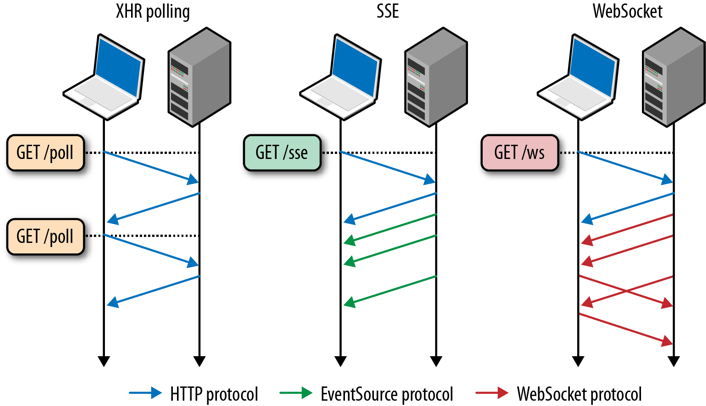
\includegraphics[width=350px]{comparativo-xhr-sse-ws.png}
	\fonte{\citeonline{grigorik2013high}}
	\label{fig:comparativo}
\end{figure}

% Alcance e contribuições

Testes de latência, realizados por \citeonline{gutwin2011real} mostraram ainda que WebSockets tem a maior taxa de transferência no envio e recebimento de mensagens através Web (Figura \ref{fig:latencia}), se mostrando, na maioria dos casos, a melhor solução para comunicação em tempo real na Web.

\begin{figure}[H]
	\centering
	\caption{Testes comparativos de latência}
	\subfloat[Cliente para servidor (500 \emph{bytes})]{
		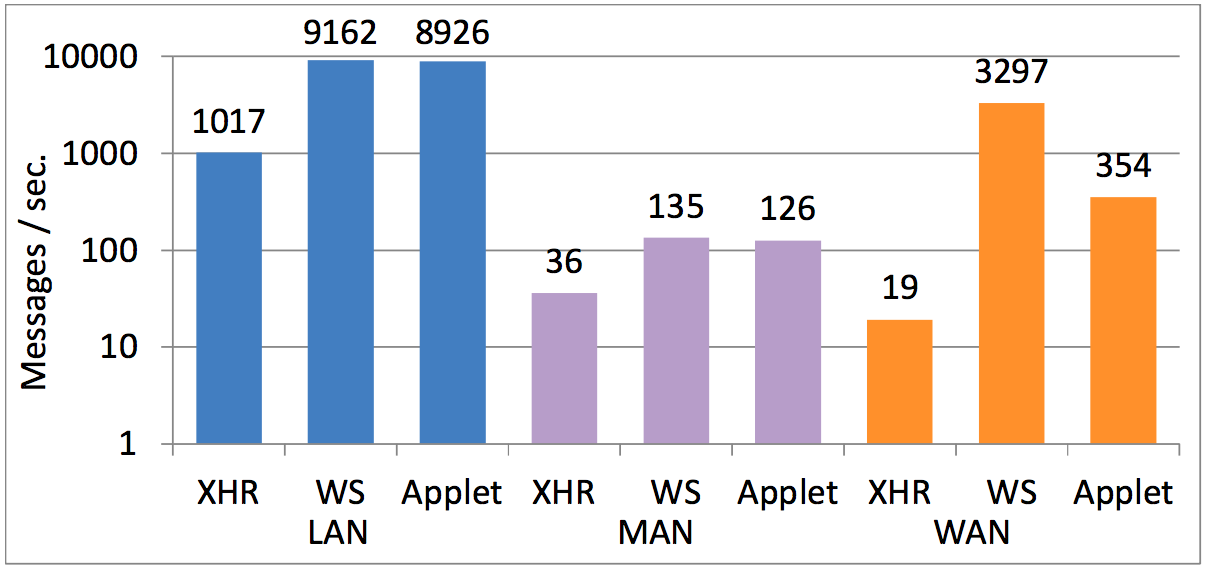
\includegraphics[width=220px]{browser-server.png}
		\label{fig:latenciarequisicao}
	}
	\hfill
	\subfloat[Servidor para cliente (500 \emph{bytes})]{
		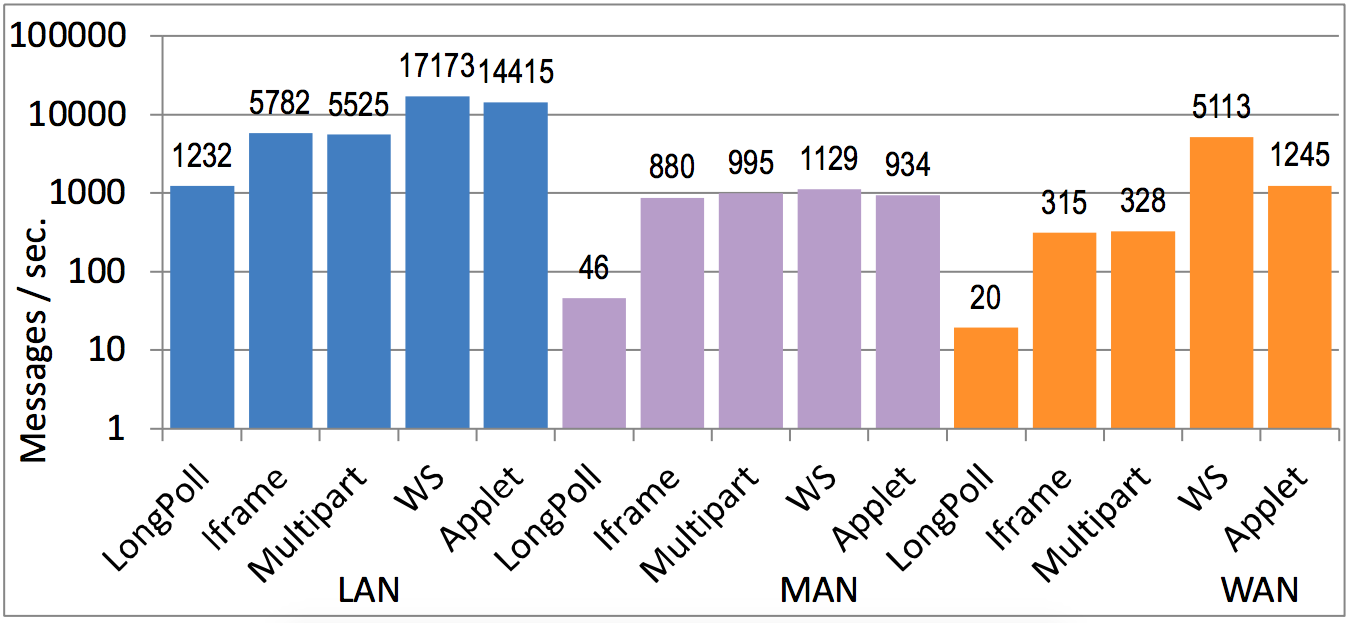
\includegraphics[width=220px]{server-browser.png}
		\label{fig:latenciaresposta}
	}
	\fonte{\citeonline{Saint-Andre2011}}
	\label{fig:latencia}
\end{figure}

Vale ressaltar que WebSocket não é um substituto para XHR ou SSE, e para o melhor desempenho é fundamental que aproveitamos os pontos fortes de cada API. Para casos onde apenas se necessita do recebimento de mensagens do servidor para o cliente (sistemas de notificações, por exemplo), SSE se mostra uma ótima escolha.